    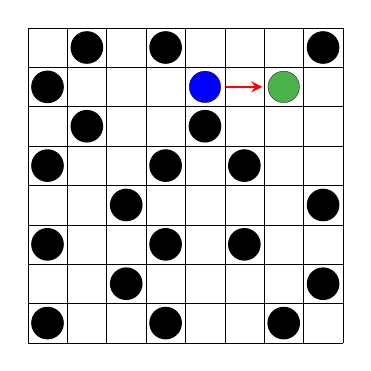
\begin{tikzpicture}
        \draw[scale = 0.5, ultra thin] ( 0,0) grid (8,8);

        % board 1 (20 replicates)
        \filldraw[black] (0.25,0.25) circle (0.2);
        \filldraw[black] (1.75,0.25) circle (0.2);
        \filldraw[black] (3.25,0.25) circle (0.2);

        \filldraw[black] (1.25,0.75) circle (0.2);
        \filldraw[black] (3.75,0.75) circle (0.2);
        
        \filldraw[black] (0.25,1.25) circle (0.2);
        \filldraw[black] (1.75,1.25) circle (0.2);
        \filldraw[black] (2.75,1.25) circle (0.2);

        \filldraw[black] (1.25,1.75) circle (0.2);
        \filldraw[black] (3.75,1.75) circle (0.2);

        \filldraw[black] (0.25,2.25) circle (0.2);
        \filldraw[black] (1.75,2.25) circle (0.2);
        \filldraw[black] (2.75,2.25) circle (0.2);

        \filldraw[black] (0.75,2.75) circle (0.2);
        \filldraw[black] (2.25,2.75) circle (0.2);
        
        \filldraw[black] (0.25,3.25) circle (0.2);
        
        \filldraw[black] (1.75,3.75) circle (0.2);
        \filldraw[black] (0.75,3.75) circle (0.2);
        \filldraw[black] (3.75,3.75) circle (0.2);

        \draw[draw = black, ultra thin, fill = blue]         (2.25,3.25) circle (0.2);
        \draw[draw = black, ultra thin, fill = green!40!gray] (3.25,3.25) circle (0.2);

        \draw[-stealth, thick, red] (2.52,3.25) -- (2.98,3.25);
    \end{tikzpicture}
